\documentclass[handout]{beamer}\mode<presentation>{\usetheme{AMSCesenaBleu}}
%\documentclass[presentation]{beamer}\mode<presentation>{\usetheme{AMSCesenaBleu}}
%%%%

\usepackage{common}
\usepackage{courses}

\title[Enviroment Setup Tutorial]{T0 -- Environment Setup Tutorial}
%
\subtitle[SD]
{Distributed Systems / Technologies\\\scriptsize Sistemi Distribuiti / Tecnologie}
%
\author[Ciatto \and Omicini]
{\alert{Giovanni Ciatto} \and \emph{Andrea Omicini}\\
\texttt{giovanni.ciatto@unibo.it \and andrea.omicini@unibo.it}}
%
\institute[DISI, Univ. Bologna]
{Dipartimento di Informatica -- Scienza e Ingegneria (DISI)\\\textsc{Alma Mater Studiorum} -- Universit{\`a} di Bologna a Cesena}
%
\date[A.Y. 2018/2019]{Academic Year 2018/2019}

\setbeamercovered{transparent}

\AtBeginSection[]
{
	\begin{frame}[c]\frametitle{Next in Line\ldots}
	%		\begin{multicols}{2}
			\tableofcontents[sectionstyle=show/shaded, subsectionstyle=show/hide, subsubsectionstyle=hide/hide]
	%		\end{multicols}
	\end{frame}
}

\begin{document}

\maketitle

\begin{frame}[c]\frametitle{Outline}
	\tableofcontents[sectionstyle=show/show, subsectionstyle=show/show, subsubsectionstyle=hide/hide]
\end{frame}

\section{Lecture goal}

\begin{frame}[allowframebreaks]
\frametitle{Lecture goal}

    \begin{itemize}
        \item In the general case it is \emph{mandatory} to \alert{use the Lab machines} when attending some Lab lesson, instead of your own laptops
        \item This is \alert{necessary} since we cannot guarantee your laptop to be properly configured 
        \item Furthermore, laptops connected to Alma-Wifi cannot directly communicate with Lab machines because of firewall rules we cannot change, thus limiting the impact of our exercises
        \item Finally, we would like to avoid wasting time configuring it \emph{during} the lesson: that time is entirely needed to present the course contents
        \item Of course, we will be glad of helping you configuring your laptops \alert{before} or \alert{after} any lecture, or by means of the \alert{students' forum} 
    \end{itemize}
    
    \framebreak
    
    \begin{itemize}
        \item In order for the Lab exercises to be reproducible on your laptops or home computers, you need to have a \alert{correctly configured environment}
        \item You must also be able to perform some basic tasks such as discovering some machine IP address or, in general, using the console
        \item This tutorial will help you configuring your computer 
        \item This tutorial will teach you some basic operations from the command line
        \item[!] Please consider reading these slides \alert{before} asking for help
        \begin{itemize}
            \item You are master students now and you can be autonomous :)
        \end{itemize}
    \end{itemize}
    
\end{frame}

\section{Lab Machines}

\subsection{In case you are using a Lab machine}

\begin{frame}
\frametitle{In case you are using a Lab machine}
    
    \columsHH{
        \begin{itemize}
            \item[!] Lab machines \alert{must} be started up choosing the \alert{\texttt{Windows 10 - Hyperv ON (x Docker)}} operative system since we may need Docker from time to time
        \end{itemize}
    }{
        \begin{center}
             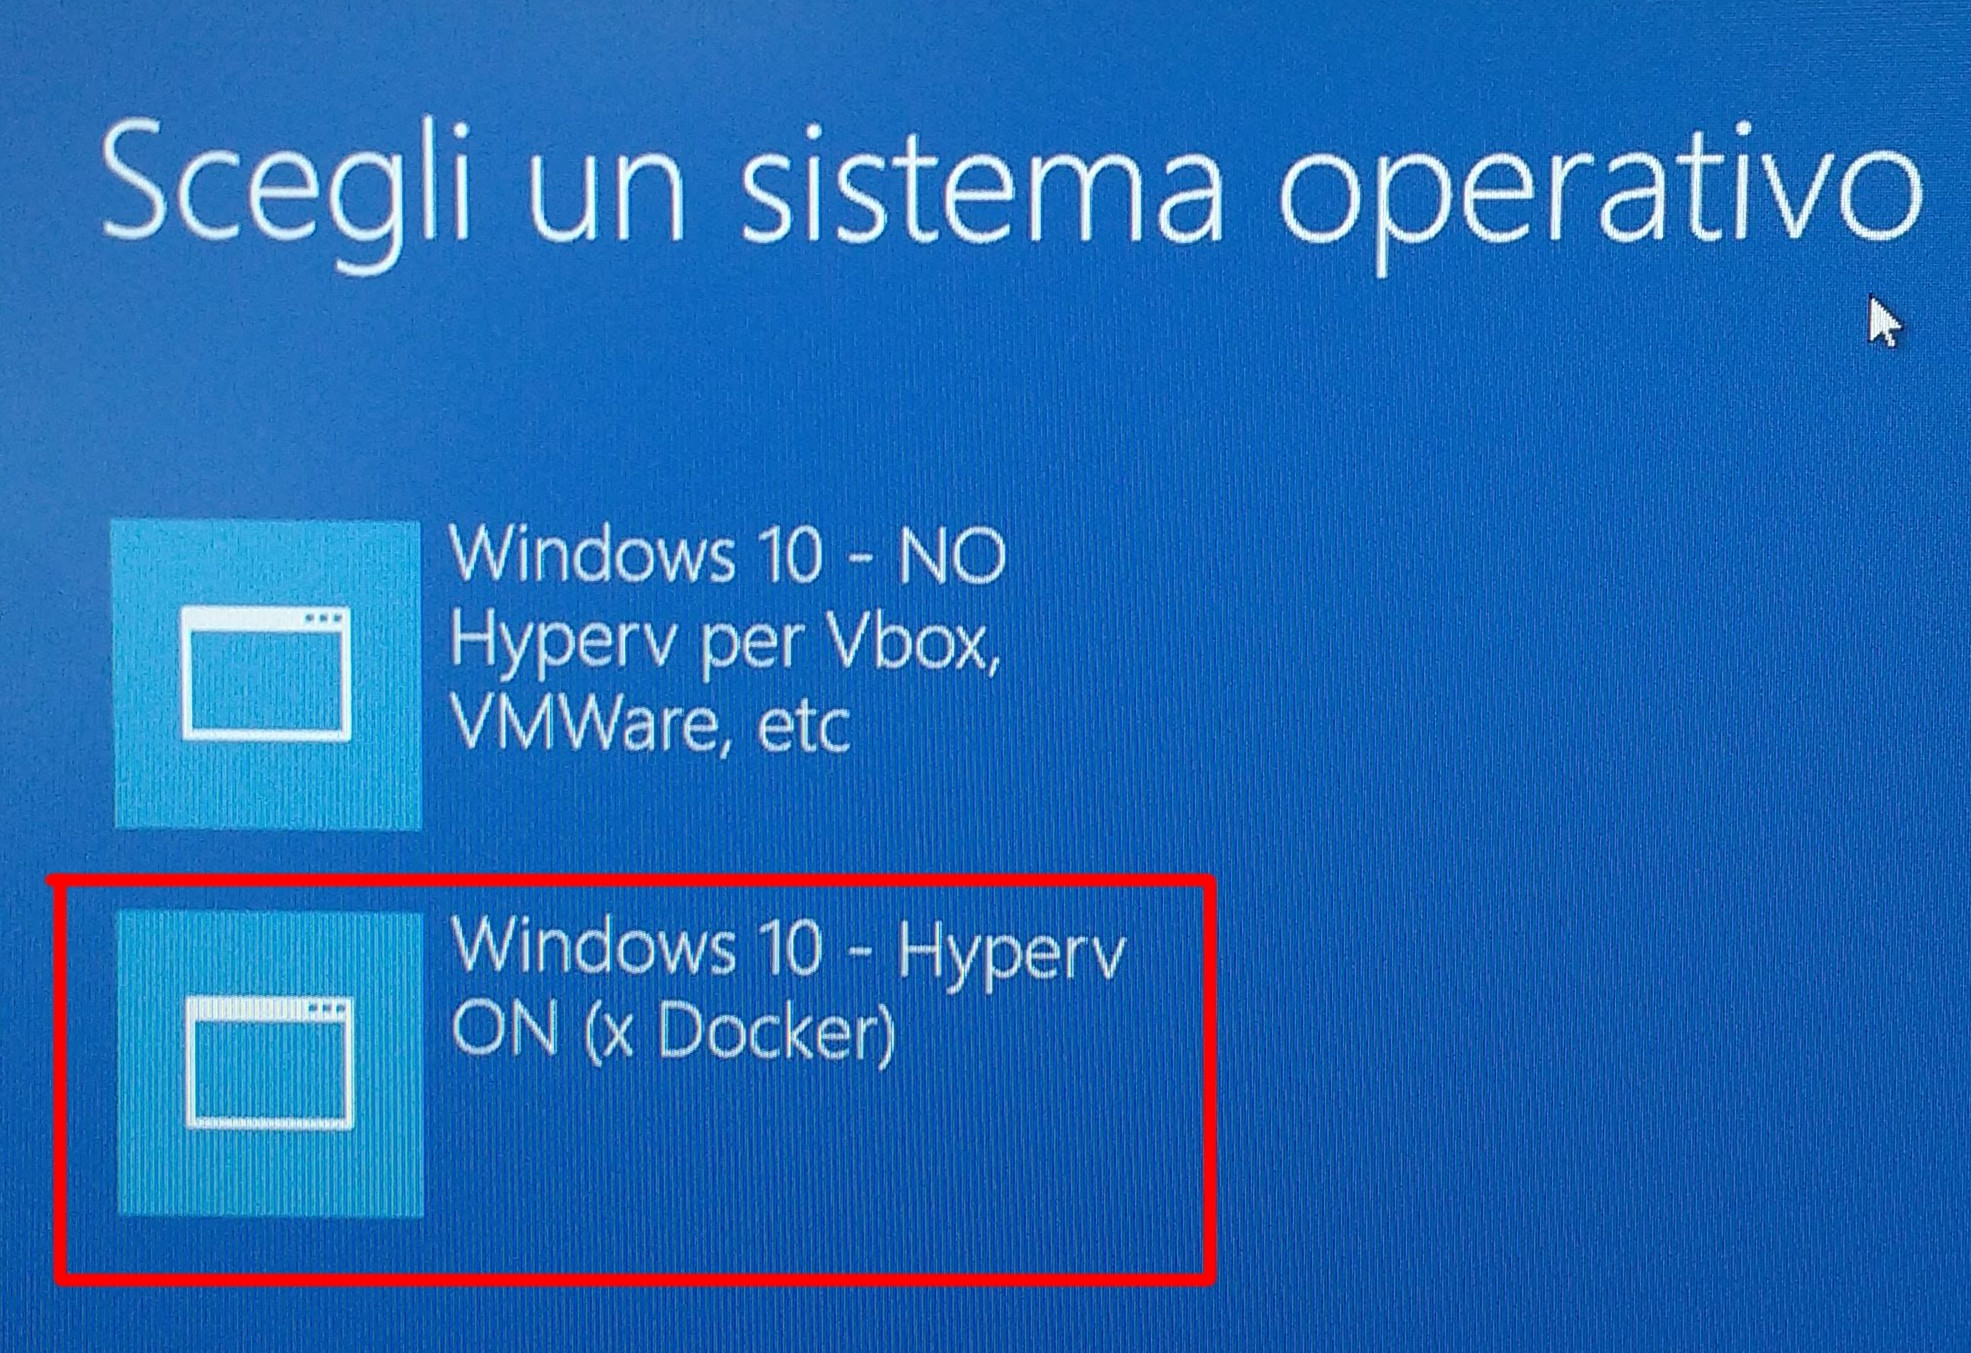
\includegraphics[width=\linewidth]{res/img/docker_so.jpg}
        \end{center}
    }
    %
    \begin{itemize}
        \item In case you are not sure whether the machine is running the right OS, please restart it---possibly, before the lecture begins

        \item In order to reduce the start up time, try keep using the same Lab machine among all Lab lectures
    \end{itemize}
    
\end{frame}

\section{Ensuring your configuration is correct}

\begin{frame}[allowframebreaks]
\frametitle{Ensuring your configuration is correct}

	\begin{enumerate}

    \item A correct configuration comprehends the following software runtimes:
    %
    \begin{itemize}
        \item \href{http://www.oracle.com/technetwork/java/javase/downloads/jdk8-downloads-2133151.html}{Java Development Kit (JDK) 8} 
        \begin{itemize}
            \item \alert{please avoid JDK versions $> 8$}
        \end{itemize}
        \item \href{https://www.docker.com/products/docker-desktop}{Docker Community Edition (CE) $\geq 17.0$}
        \item \href{https://gradle.org/releases}{Gradle $\geq 4.0.0$}
        \item \href{https://git-scm.com}{Git $\geq 2.15.0$}
    \end{itemize}

	\item Ensure they are installed or install them if they are not
	%
	\begin{itemize}
		\item Notice that Gradle required Java to be installed
		\item Notice that, on Windows, Docker requires \alert{Hyper-V} to be enabled 
		%
		\begin{itemize}
			\item Notice that Hyper-V is NOT supported by Windows 10 Home
			\item Consider reading slide \ref{troubleshooting}
		\end{itemize}
	\end{itemize}
    
    \framebreak
    
    \item If your configuration is correct, the following commands should provide an output similar to the one shown in this slide:
    %
    \begin{itemize}
        \item[\$] \texttt{java -version}
        \begin{itemize}
            \item[$\rightarrow$] \texttt{java version "1.8.X\_Y"}
            \item[] \texttt{Java(TM) SE Runtime Environment (build 1.8.X\_Y)}
            \item[] \texttt{Java HotSpot(TM) 64-Bit Server VM ZZZ}
        \end{itemize}
        
        \item[\$] \texttt{javac -version}
        \begin{itemize}
            \item[$\rightarrow$] \texttt{javac 1.8.X\_Y}
        \end{itemize}
        
        \item[\$] \texttt{gradle --version}
        \begin{itemize}
            \item[$\rightarrow$] \texttt{Gradle 4.X.Y}
            \item[] \ldots
        \end{itemize}
        
        \item[\$] \texttt{docker --version}
        \begin{itemize}
            \item[$\rightarrow$] \texttt{Docker version 17.X.Y-ce, build ZZZ}
        \end{itemize}
        
        \item[\$] \texttt{git --version}
        \begin{itemize}
            \item[$\rightarrow$] \texttt{git version 2.15.X.Y}
        \end{itemize}
    \end{itemize}
	%
	\framebreak
    %
    For instance, on Windows:
    %
    \begin{center}
        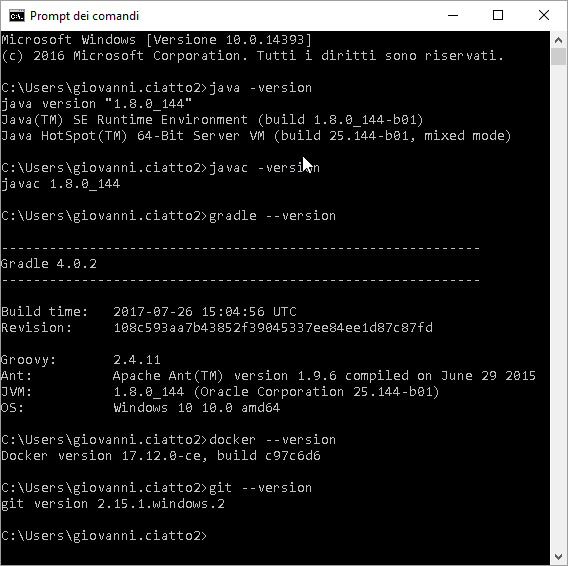
\includegraphics[width=.4\linewidth]{res/img/console_versions.png}
    \end{center}
    %
    \alert{If you get any trouble}, ensure the aforementioned software is correctly installed AND the following environment variables are properly set.
    
    \framebreak
    
    \item You must ensure the \texttt{JAVA\_HOME} and \texttt{GRADLE\_HOME} environment variables are properly set
    %
    \begin{itemize}
    	\item they should respectively point to the paths where \texttt{JDK} and Gradle are installed
    \end{itemize}
    
    \vspace{.5cm}
    
    \item For instance, you can check them by running the following console commands:
    %
    \begin{itemize}
        \item[$>$] \texttt{echo \alert{\%}JAVA\_HOME\alert{\%} \& echo \alert{\%}GRADLE\_HOME\alert{\%}}
        \begin{itemize}
            \item[$\rightarrow$] \texttt{C:$\backslash$Program Files$\backslash$Java$\backslash$jdk\_1.8.X\_Y} \hint{your paths may}
            \item[] \texttt{C:$\backslash$Program Files$\backslash$Gradle$\backslash$gradle-4.X.Y} \hint{be different}
        \end{itemize}
    \end{itemize}
    %
    on Windows-based systems, or
    %
    \begin{itemize}
        \item[\$] \texttt{echo \alert{\$}JAVA\_HOME ; echo \alert{\$}GRADLE\_HOME}
        \begin{itemize}
            \item[$\rightarrow$] \texttt{/usr/lib/jvm/java-8-openjdk-amd64/}\hint{your paths may}
            \item[] \texttt{/opt/gradle/gradle-4.X.Y}\hint{be different}
        \end{itemize}
    \end{itemize}
    %
    on Unix-based systems.
    
   \framebreak
    
   \item Then, you must ensure your \texttt{PATH} environment variable contains the paths  where the aforementioned runtimes are installed into. 
	%
	\begin{itemize}
		\item[!] If you succeeded with the previous steps, this should be ok, but please double check :)
	\end{itemize}
	%    
    \vspace{.5cm}
    %
    For instance, you can check it by running the following console commands:
    %
    \begin{itemize}
        \item[$>$] \texttt{echo \alert{\%}PATH\alert{\%}}
        \begin{itemize}
            \item[$\rightarrow$] \texttt{<path1>}\alert{;}\texttt{<path2>}\alert{;}$\ldots$\alert{;}\textit{\texttt{<java\_home>$\backslash$bin}}\alert{;}$\ldots$\alert{;}\textit{\texttt{<gradle\_home>$\backslash$bin}}\alert{;}$\ldots$
        \end{itemize}
    \end{itemize}
    %
    on Windows-based systems, or
    %
    \begin{itemize}
        \item[\$] \texttt{echo \alert{\$}PATH}
        \begin{itemize}
            \item[$\rightarrow$] \texttt{<path1>}\alert{:}\texttt{<path2>}\alert{:}$\ldots$\alert{:}\textit{\texttt{<java\_home>/bin}}\alert{:}$\ldots$\alert{:}\textit{\texttt{<gradle\_home>/bin}}\alert{:}$\ldots$
        \end{itemize}
    \end{itemize}
    %
    on Unix-based systems.
    
    \framebreak
    
    \item Ensure your local Git properties \alert{\texttt{user.name}} and \alert{\texttt{user.email}} are properly set by running the following commands:
    %
    \begin{itemize}	
    	\item[\$] \texttt{git config --global --get user.\alert{name}}
    	%
    	\begin{itemize}	
    		\item[$\rightarrow$] \texttt{\textit{<your name>}}    		
    	\end{itemize}
    	
    	\item[\$] \texttt{git config --global --get user.\alert{email}}
    	%
    	\begin{itemize}	
    		\item[$\rightarrow$] \texttt{\textit{<name>}.\textit{<surname>}[\textit{<number>}]@\alert{studio.unibo.it}}    		
    	\end{itemize}
    
    	\vspace{.5cm}
    	
    	\item In case they are not, you can set them by means of the following command
    	%
    	\begin{itemize}	
    		\item[\$] \texttt{git config --global \texttt{\textit{<property\_name>}} \alert{"}\texttt{\textit{<value>}}\alert{"}}		
    	\end{itemize}
    \end{itemize}
    
    \framebreak
    
    \item Ensure, the Docker service/daemon is up and running
    %
    \begin{itemize}
       	\item on Windows and Mac OS, this just means checking the Docker icon is present within the taskbar 
		%
		\columsHH{
			
\includegraphics[width=.9\linewidth]{./res/img/docker_icon_win.png}
			
		}{
			
\includegraphics[width=.9\linewidth]{./res/img/docker_icon_mac.png}
		}
	
		\vspace{.3cm}
	
		\item on Linux, you need to execute one of the following commands:
		%
		\begin{itemize}
			\item[\$] \texttt{service docker status}
			\item[] or
			\item[\$] \texttt{systemctl status docker.service}
		\end{itemize}
		
		\item in case the Docker service is NOT up and running, you can start it by running:
		
		%
		\begin{itemize}
			\item[\$] \texttt{\alert{sudo} service docker start}
			\item[] or
			\item[\$] \texttt{\alert{sudo} systemctl start docker.service}
		\end{itemize}
	\end{itemize}
    
    \framebreak
    
    \item Finally, you must check if Docker is currently logged in with your Docker Hub credentials
    %
    \begin{itemize}
    	\item this requires you registered on \url{https://hub.docker.com/} as explained on slide \ref{configure-accounts}
    \end{itemize}
   	%
    \vspace{.5cm}
    %
    For instance, you can do so by running the following console commands:
    %
    \begin{itemize}
        \item[$>$] \texttt{docker login}
        \begin{itemize}
            \item If you get an output like the following one, then your Docker is already logged in. 
            Press \alert{Ctrl+C} to stop the current login procedure.
            
            \vspace{.3cm}
            
            \item[$\rightarrow$] \texttt{Login with your Docker ID to push and pull images from Docker Hub. If you don't have a Docker ID, head over to https://hub.docker.com to create one.}
            \item[] \texttt{Username (\alert{your\_username}):}
            
            \vspace{.3cm}
            
            \item Otherwise, if no \texttt{(\alert{your\_username})} part is readable or if the prompted username is not yours, go on typing your Docker ID \& password
        \end{itemize}
    \end{itemize}
    %
    \framebreak
    %
    Example:
    %
    \vspace{.3cm}
    %
    \columsHH{
        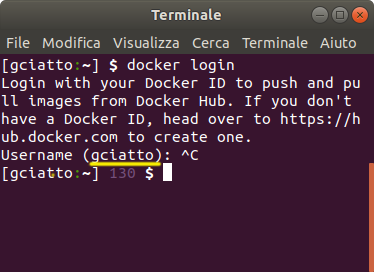
\includegraphics[width=\linewidth]{res/img/docker_logged.png}
        
        Logged
    }{
        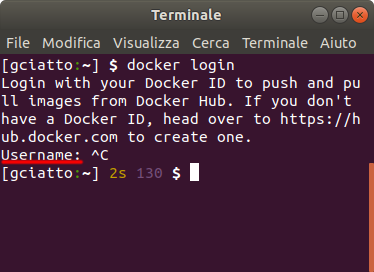
\includegraphics[width=\linewidth]{res/img/docker_unlogged.png}
        
        Not logged
    }
	\end{enumerate}

\end{frame}

\section{Create the required accounts}

\begin{frame}\label{configure-accounts}
\frametitle{Create the required accounts}
    
    For this course, you will need to:
    %
    \begin{enumerate}
        \item Be enrolled into the course e-learning web-page
        \begin{itemize}
            \item \url{https://iol.unibo.it/enrol/index.php?id=23794}
            \item you should be already enrolled because of your courses plan
            \item if you are not, you can enroll providing the key \alert{\texttt{1819SD}}
        \end{itemize}
        
        \item Register a GitLab account using your \alert{\texttt{x.yN@studio.unibo.it}} email address
        \begin{itemize}
            \item \url{https://gitlab.com/users/sign_in\#register-pane}
            \item please use \texttt{x.yN} as username, if possible
        \end{itemize}
        
        \item Register a Docker Hub account using your \alert{\texttt{x.yN@studio.unibo.it}} email address
        \begin{itemize}
            \item \url{https://hub.docker.com/}
            \item please use \texttt{xyN} as Docker ID, if possible
        \end{itemize}
        
        \item Request access on the Distributed Systems GitLab group for the A.Y. 2018/2019:
        %
        \begin{itemize}
            \item \url{https://gitlab.com/das-lab/courses/ds/aa1819}
        \end{itemize}
        
    \end{enumerate}
    
\end{frame}

\section{Operations}

\subsection{Importing your (Git) project in Eclipse}

\begin{frame}[allowframebreaks]
\frametitle{Importing your (Git) project in Eclipse} 
    Suppose you want to import your Git \texttt{http://gitwhatever.com/path/to/\alert{my-project}} project in Eclipse:
    %
    \begin{enumerate}
        \item Clone your project within the \texttt{\alert{my-dir}} directory:
        %
        \begin{itemize}
            \item[!] Ensure \texttt{my-dir} is NOT an Eclipse workspace
            \item[\$] \texttt{cd \alert{my-dir}}
            \item[\$] \texttt{git clone http://gitlab.com/path/to/X} 
        \end{itemize}
        
        \item \textbf{Start Eclipse and choose \texttt{\alert{my-dir}} as the workspace directory}
        
        \item Import the existing project into the workspace, if possible:
        %
        \begin{enumerate}
            \item Click on \texttt{File} a menu should appear
            \item Click on \texttt{Import...} a dialog window should appear
            \item From that dialog, open the \texttt{General} folder
            \item Select the \texttt{Existing Projects into Workspace} and click on \texttt{Next}
            \item Ensure the \texttt{Select root directory} field is selected
            \item Click on the \texttt{Browse...} button and select the \texttt{\alert{my-dir}} directory (i.e.,  the current workspace)
            \item If your cloned project \texttt{\alert{my-project}} is visible within the \texttt{Projects} area, select it and hit the \texttt{Finish} button
            \item Otherwise, Git is not tracking Eclipse's project files and you must import the project the hard way (next step)
        \end{enumerate}
        
        \item If the previous procedure fails, close the \texttt{Import} dialog and
        %
        \begin{enumerate}
            \item Click on \texttt{File} a menu should appear
            \item Select the \texttt{New > Java Project} entry
            \item Type \texttt{\alert{my-project}} within the \texttt{Project name} field
            \item Hit the \texttt{Finish} button
        \end{enumerate}
        
        \item If no procedure succeeded you can call for help :)
        
    \end{enumerate}
\end{frame}

\subsection{Submitting your weekly exercise}

\begin{frame}%[allowframebreaks]
\frametitle{Submitting your weekly exercise}

    \begin{itemize}

        \item Sometimes, you will be asked to solve some exercises
        
        \item You will usually clone them from a GitLab repository and \alert{submit your solutions to the same repository}
        \begin{itemize}
            \item So please request access here: \url{https://gitlab.com/das-lab/courses/ds/aa1819} in order to get the right to push your commits
        \end{itemize}
        
        \item Your will be required to push your solution on the following \alert{branch}:
        \begin{itemize}
            \item \texttt{submissions/\alert{\textit{name.surnameN}}}, in case you are submitting on time
            \item \texttt{late-submissions/\alert{\textit{name.surnameN}}}, otherwise
            
            \vspace{.3cm}
        
            \item[!] The definition of ``on time'' may vary but it usually means ``before the next Lab lecture''
            
            \item[!] Of course, your push right on the \texttt{submissions/*} branches will eventually be deactivated
            
            \vspace{.3cm}
            
            \item[$\downarrow$] Example on the next slide

        \end{itemize}

    \end{itemize}
\end{frame}

\begin{frame}[allowframebreaks]
\frametitle{Exercise workflow example}

    \begin{enumerate}
        \item Clone the exercise repository
        %
        \begin{itemize}
            \item[\$] \texttt{git clone https://gitlab.com/das-lab/courses/ds/aa1819/\alert{\textit{exericse\_name}}}
        \end{itemize}
        
        \item Jump into the project directory
        %
        \begin{itemize}
            \item[\$] \texttt{cd \alert{\textit{exericse\_name}}}
        \end{itemize}
        
        \item Create a novel submission branch:
        %
        \begin{itemize}
            \item[\$] \texttt{git checkout -b submissions/\textit{\alert{name.surnameN}}}
        \end{itemize}
        
        \item Repeat until exercise completion:
        %
        \begin{enumerate}
            \item Do some work
            \item Add the edited files to the stage
            %
            \begin{itemize}
                \item[\$] \texttt{git add \textit{\alert{edited\_file1}}, \textit{\alert{edited\_file1}}, \ldots}
            \end{itemize}
            \item Commit the staged files 
            %
            \begin{itemize}
                \item[\$] \texttt{git commit -m "\textit{\alert{a message here}}"}
            \end{itemize}
            \item Push on the \texttt{submissions/\textit{\alert{name.surnameN}}} branch
            %
            \begin{itemize}
                \item[\$] \texttt{git \alert{push}}
            \end{itemize}
        \end{enumerate}
        
        \item In case your push fails, you may be out of time. You can create a \texttt{late-submissions/*} branch by running:
        %
        \begin{itemize}
            \item[\$] \texttt{git checkout -b late-submissions/\textit{\alert{name.surnameN}}}
            
            \vspace{.3cm}
            
            \item And, again, you can push on the \texttt{late-submissions/\textit{\alert{name.surnameN}}} branch by running:
            %
            \begin{itemize}
                \item[\$] \texttt{git \alert{push}}
            \end{itemize}
        \end{itemize}
        
        \item If your push fails, and you are on time, quickly contact the tutor by means of the forum
            
    \end{enumerate}

\end{frame}

\subsection{Discovering your machine IP address}

\begin{frame}[allowframebreaks]
\frametitle{Discovering your machine IP address(es)} 


	In several scenarios you may be required to discored your machine current IP address
	%
	\columnsHHt{
		\begin{itemize}
		    \item On Windows, you can do it by prompting:
		    %
		    \begin{itemize}
		        \item[$>$] \texttt{ipconfig}
		    \end{itemize}
		\end{itemize}
		%
		\begin{center}
			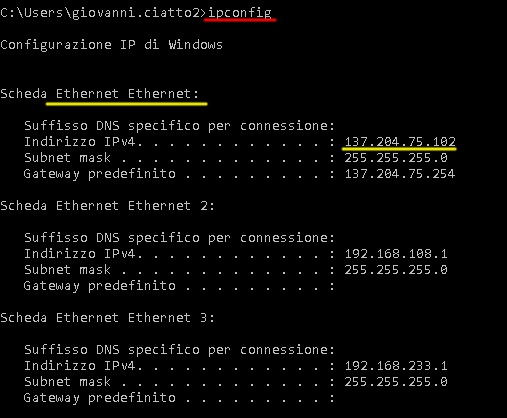
\includegraphics[width=.9\linewidth]{res/img/ipconfig.png}
		\end{center}
	}{%\framebreak
    \begin{itemize}
	    \item Whereas, on Unix, you can do it by prompting:
	    %
	    \begin{itemize}
	        \item[\$] \texttt{ifconfig}
	    \end{itemize}
	\end{itemize}
	%
	\begin{center}
		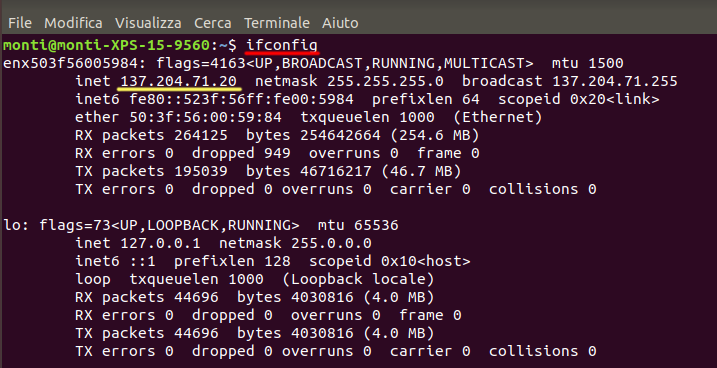
\includegraphics[width=.9\linewidth]{res/img/ifconfig.png}
	\end{center}
	}
    
    \framebreak
    \begin{itemize}
    \item Keep in mind that:
    %
    \begin{itemize}
    	\item IP addresses are often dynamically assigned by means of DHCP, so \alert{do not expect} you machine to always be assigned with the same IP address
    	\item IP addresses are usually NATted, thus they are not accessible from the Internet
    	\item UniBo's IP addresses are \emph{usually} in the \texttt{137.204.xx.xx} form
    	\item Docker \emph{usually} assign IPs to containers in from the \texttt{172.xx.xx.xx} range
    \end{itemize}
	\end{itemize}

\end{frame}

\subsection{Configure your own computer}

\begin{frame}
\frametitle{Configure your own computer}

	Some useful tutorials:
	%
	\begin{itemize} 
		
		\item \href{https://docs.gradle.org/current/userguide/installation.html\#installing_manually}{How to install Gradle on Windows, Mac OS, or Linux}
		
		\item How to install Docker...
		%
		\begin{itemize}
			\item \ldots{} \href{https://docs.docker.com/docker-for-mac/install/}{on Mac OS} or \href{https://docs.docker.com/docker-for-windows/install/}{on Windows}
			\item \ldots{} on Linux \href{https://docs.docker.com/install/linux/docker-ce/centos/}{CentOS}, \href{https://docs.docker.com/install/linux/docker-ce/debian/}{Debian}, \href{https://docs.docker.com/install/linux/docker-ce/fedora/}{Fedora}, \href{https://docs.docker.com/install/linux/docker-ce/ubuntu/}{Ubuntu}, or \href{https://docs.docker.com/install/linux/docker-ce/binaries/}{other distributions}
			%
			\begin{itemize}
				\item \href{https://docs.docker.com/install/linux/linux-postinstall/}{Some further configuration steps for Linux}
			\end{itemize}
		\end{itemize}
		
		\item	 \href{https://confluence.atlassian.com/doc/setting-the-java_home-variable-in-windows-8895.html}{Hot to set the \texttt{JAVA\_HOME} environment variable on Windows}
		%
		\begin{itemize}
			\item Other environment variables can be set in a similar way
		\end{itemize}
		
		\item \href{https://www.java.com/en/download/help/path.xml}{How to edit the \texttt{PATH} environment variable on Windows or Mac OS}
		%
		\begin{itemize}
			\item Instructions for Mac OS are ok for Linux too
		\end{itemize}
	
		\item \href{https://docs.microsoft.com/it-it/virtualization/hyper-v-on-windows/quick-start/enable-hyper-v}{How to enable Hyper-V on Windows}
	
		\item \href{https://git-scm.com/book/en/v2/Customizing-Git-Git-Configuration}{How to set up Git properties}
	\end{itemize}

	\begin{block}{}
		In case of troubles, you can post on the \href{https://iol.unibo.it/mod/forum/view.php?id=123707}{Students' Forum} \alert{describing your issues}, your computer's features, and the steps you already performed :)
	\end{block}

\end{frame}

\subsection{Troubleshooting}

\begin{frame}\label{troubleshooting}
\frametitle{Troubleshooting} 
	\begin{itemize}
		\item In case your PC runs Windows 10 Home or some former version of Windows, you can freely and legally get a Windows 10 Pro license \& self-installing image since you are an UniBo student
		%
		\begin{itemize}
			\item You must apply to \href{https://dreamspark.campusfc.unibo.it/}{UniBo's Microsoft Programme}
			\item It may require a few days for your account to be activated 
		\end{itemize}
	
		\vspace{.3cm}
	
		\item For other sorts of troubles, please create a post on the \href{https://iol.unibo.it/mod/forum/view.php?id=123707}{Students' Forum}
		
%		\item If you feel shy, you can also post your questions on the \href{https://docs.google.com/document/d/1Nk3h5wPtEVD_GXjdmfBGjJpdDnqPIo1IJhArUh4oGS4/edit}{Anonymous Questions Blackboard}
	\end{itemize}
\end{frame}

\maketitle

%%%%%%%%%%%%%%%%%%%%%%%%%%%%%%%%%%%%%%%%%%%%%%%%%%%%%%%%%%%%%%%%%%%%%%%%%%%%%%%
\end{document}
%%%%%%%%%%%%%%%%%%%%%%%%%%%%%%%%%%%%%%%%%%%%%%%%%%%%%%%%%%%%%%%%%%%%%%%%%%%%%%%%